\documentclass{ctexart}
\usepackage{amsmath, amsfonts, amssymb} % 数学公式、符号
\usepackage[colorlinks,linkcolor=red,anchorcolor=blue,citecolor=green]{hyperref}
\usepackage[left=2.50cm, right=2.50cm, top=2.50cm, bottom=2.50cm]{geometry} %页边距
\usepackage{graphicx}   % 图片
\usepackage{multicol}
\usepackage{bm}
\usepackage{listings}
\usepackage{xcolor}
\usepackage{tikz}
\usetikzlibrary{arrows,shapes,chains}
\usepackage{multirow}
\usepackage{algorithm}  
\usepackage{algpseudocode}  

\floatname{algorithm}{算法}
\renewcommand{\algorithmicrequire}{\textbf{输入:}}  % Use Input in the format of Algorithm  
\renewcommand{\algorithmicensure}{\textbf{输出:}} % Use Output in the format of Algorithm
\usepackage{fancyhdr} %设置页眉、页脚
\pagestyle{fancy}
% 用来设置代码的样式
\lstset{
	basicstyle          =   \sffamily,          % 基本代码风格
	keywordstyle        =   \bfseries,          % 关键字风格
	commentstyle        =   \rmfamily\itshape,  % 注释的风格,斜体
	stringstyle         =   \ttfamily,  % 字符串风格
	flexiblecolumns,                % 别问为什么,加上这个
	numbers             =   left,   % 行号的位置在左边
	showspaces          =   false,  % 是否显示空格,显示了有点乱,所以不现实了
	numberstyle         =   \zihao{-5}\ttfamily,    % 行号的样式,小五号,tt等宽字体
	showstringspaces    =   false,
	captionpos          =   t,      % 这段代码的名字所呈现的位置,t指的是top上面
	frame               =   lrtb,   % 显示边框
}

\lstdefinestyle{Python}{
	language        =   Python, % 语言选Python
	basicstyle      =   \zihao{-5}\ttfamily,
	numberstyle     =   \zihao{-5}\ttfamily,
	keywordstyle    =   \color{blue},
	keywordstyle    =   [2] \color{teal},
	stringstyle     =   \color{magenta},
	commentstyle    =   \color{red}\ttfamily,
	breaklines      =   true,   % 自动换行,建议不要写太长的行
	columns         =   fixed,  % 如果不加这一句,字间距就不固定,很丑,必须加
	basewidth       =   0.5em,
}

\title{\textbf{机器学习实验报告\\{\Large{决策树}}}} % 标题与子标题
\author{\sffamily{朱天泽}} % 作者
\date{(日期:\today)} % 日期
\setlength{\abovecaptionskip}{0.1cm}
\begin{document}
	\maketitle
	% 摘要开始
	\noindent{\bf{摘要}}
	在《机器学习》第四章中,我学习了决策树模型。在此次实验中,我尝试用DFS和BFS实现了多个用于分类任务的决策树模型,包括针对离散值的单变量决策树、基于对数几率回归的多变量决策树。在训练好决策树模型的基础上,我使用了4个UCI数据集,比较了未剪枝、预剪枝、后剪枝三种类型决策树的准确率。此外,我尝试使用了机器学习库scikit-learn,同自己实现的算法进行了比较。
	
	\noindent{\bf{关键词}} 决策树;剪枝;分类;搜索;scikit-learn
	
	% 正文开始
	\section{习题1}
	\subsection{编程题目理解}
	题目要求:任意选择4个UCI数据集,对基于信息增益划分选择(ID3)、基于基尼指数划分选择(CART),基于对率回归划分选择的决策树算法(包括未剪枝、预剪枝、后剪枝三种)进行实验比较。
	
	ID3、CART两种划分选择,可用于实现单变量的决策树;对率回归是一个线性分类模型,基于对率回归,可以实现多变量决策树。在实现未剪枝决策树的基础上,还需要对决策树进行前剪枝或后剪枝。
	
	\subsection{决策树模型原理阐述}
	\subsubsection{决策树构建过程}
	一般的,一棵决策树包含一个根结点、若干个内部结点和若干个叶结点;叶结点对应于决策结果,其它每个结点则对应于一个属性测试;每个结点包含的样本集合根据属性测试的结果被划分到子结点中;根结点包含样本全集。从根结点到每个叶结点的路径对应了一个判定测试序列。决策树学习的目的是为了产生一棵泛化能力强,即处理未见示例能力强的决策树,其基本流程遵循简单且直观的“分而治之”策略。
	
	\begin{algorithm}[!htb]
		\caption{决策树学习基本算法}  
		\label{决策树学习基本算法}
		\begin{algorithmic}[1]
			\Require  
			训练集 $D=\{(\bm{x}_1,y_1),(\bm{x}_2,y_2),\cdots,(\bm{x}_m,y_m)\}$;属性集 $A=\{a_1,a_2,\cdots,a_d\}$。
			\Ensure
			决策树的根节点root
			\Function{TreeGenerate}{$D$, $A$}
			生成结点node;
			\If{$D$ 中样本全属于同一类别 $C$}
				\State 将node标记为 $C$ 类叶结点;
				\Return
			\EndIf
			\If{$A\neq\varnothing$ \textbf{OR} $D$ 中样本在 $A$ 上取值相同}
				\State 将node标记为叶结点,其类别标记为 $D$ 中样本最多的类;
				\Return
			\EndIf
			\State 从 $A$ 中选择最优划分属性 $a_\ast$;
			\For{$a_\ast$的每个值 $a_\ast^v$}
				\State 为node生成一个分支;令 $D_v$ 表示 $D$ 中在 $a_\ast$ 上取值为 $a_\ast^v$ 的样本子集;
				\If{$D_v$为空}
					\State 将分支结点标记为叶结点,其类别标记为 $D$ 中样本最多的类;
					\Return
				\Else
					\State 以 \Call{TreeGenerate}{$D_v$, $A\ \backslash\ \{a_\ast\}$} 为分支结点
				\EndIf
			\EndFor
			\EndFunction
		\end{algorithmic}  
	\end{algorithm}

	就如算法\ref{决策树学习基本算法},决策树的生成是一个递归过程。在决策树基本算法中,有三种情形会导致递归返回:
	
	\begin{enumerate}
		\item 当前节结点包含的样本全属于同一类别,无需划分;
		\item 当前属性集为空,或是所有样本在所有属性上取值相同,无法划分;
		\item 当前节点包含的样本集合为空,不能划分。
	\end{enumerate}

	在第2种情形下,我们把当前结点标记为叶结点,并将其类别设定为该结点所含样本最多的类别;在第3种情形下,同样把当前结点标记为叶结点,但将其类别设定为其父结点所含样本最多的类别。这两种情形的处理有实质不同:情形2是在利用当前结点的后验分布,而情形3则是把父结点的样本分布作为当前结点的先验分布。
	
	\subsubsection{划分选择}
	
	由算法\ref{决策树学习基本算法}可以看出,决策树学习的关键是如何选择最优划分属性。一般而言,随着划分过程不断进行,我们希望决策树的分支结点所包含的样本尽可能属于同一类别,即结点的“纯度”越来越高。在本次实验,我实现了基于信息增益和基尼指数的决策树。
	
	\paragraph{信息增益} ID3决策树学习算法以信息增益为准则来选择划分属性。

	信息熵是度量样本集合纯度最常用的一种指标。假定当前样本集合 $D$ 中第 $k$ 类样本所占的比例 $p_k\ (k=1,2,\cdot,|\mathcal{Y}|)$,则 $D$ 的信息熵定义为
	
	\begin{equation}
		\operatorname{Ent}(D)=-\sum_{k=1}^{|\mathcal{Y}|} p_{k} \log _{2} p_{k}
		\label{Ent}
	\end{equation}

	$\operatorname{Ent}(D)$ 的值越小,则 $D$ 的纯度越高。
	
	假定离散属性 $a$ 有 $V$ 个可能的取值 $\{a^1,a^2,\cdots,a^V\}$,若使用 $a$ 来对样本集 $D$ 进行划分,则会产生 $V$ 个分支结点,其中第 $v$ 个分支结点包含了 $D$ 中所有在 $a$ 取值上为 $a^v$ 的样本,记为 $D^v$。我们可根据式\eqref{Ent}计算出 $D^v$ 的信息熵,再考虑到不同的分支结点所包含的样本数不同,给分支结点赋予权重 $\frac{|D^v|}{|D|}$,即样本数越多的分支结点的影响越大,于是可计算出用属性 $a$ 对样本集 $D$ 进行划分所获得的“信息增益”
	
	\begin{equation}
		\operatorname{Gain}(D, a)=\operatorname{Ent}(D)-\sum_{v=1}^{V} \frac{\left|D^{v}\right|}{|D|}\operatorname{Ent}\left(D^{v}\right)
		\label{Gain}
	\end{equation}

	一般而言,信息增益越大,则意味着使用属性 $a$ 来进行划分所获得的“纯度提升”越大。因此,我们可用信息增益来进行决策树的划分属性选择,即在算法\ref{决策树学习基本算法}中,$a_\ast=\underset{a \in A}{\arg \max } \operatorname{Gain}(D, a)$。
	
	\paragraph{基尼指数} CART决策树使用“基尼指数”来选择划分属性。
	
	采用与式\eqref{Ent}相同的符号,数据集 $D$ 的纯度可用基尼值来度量:
	
	\begin{equation}
		\begin{aligned}
			\operatorname{Gini}(D) &=\sum_{k=1}^{|\mathcal{Y}|} \sum_{k^{\prime} \neq k} p_{k} p_{k^{\prime}} \\
			&=1-\sum_{k=1}^{|\mathcal{Y}|} p_{k}^{2}
		\end{aligned}
	\end{equation}

	直观来说,$\operatorname{Gini}(D)$ 反映了从数据集 $D$ 中随机抽取两个样本,其类别标记不一致的概率。因此,$\operatorname{Gini}(D)$ 越小,则数据集 $D$ 的纯度越高。
	
	采用与式\eqref{Gain}相同的符号表示,属性 $a$ 的基尼指数定义为
	
	\begin{equation}
		\operatorname{Gini\_index}(D, a)=\sum_{v=1}^{V} \frac{\left|D^{v}\right|}{|D|} \operatorname{Gini}\left(D^{v}\right)
	\end{equation}

	于是,我们在候选属性集合 $A$ 中,选择那个是的划分后基尼指数最小的属性作为最优划分属性,即 
	
	\begin{equation}
		a_\ast=\underset{a \in A}{\arg \min } \operatorname{Gini\_index}(D, a)
	\end{equation}
	
	\subsubsection{剪枝处理}
	
	在决策树学习中,为了尽可能正确分类训练样本,结点划分过程将不断重复,有时会造成决策树分支过多,以致于把训练集自身的一些特点当作所有数据都具有的一般性质而导致过拟合。因此,可通过主动去掉一些分支来降低过拟合的风险。
	
	决策树剪枝的基本策略有“预剪枝”和“后剪枝”。预剪枝是指在决策树生成过程中,对每个结点在划分前先进行估计,若当前结点的划分不能带来决策树泛化性能提升,则停止划分并将当前结点标记为叶结点;后剪枝则是先从训练集生成一棵完整的决策树,然后自底向上地对非叶结点进行考察,若将该结点对应的子树替换为叶结点能带来决策树泛化性能提升,则将该子树替换为叶结点。
	
	决策树的泛化性能需要使用测试集来评估,在预剪枝和后剪枝的过程中,若添加或删除结点能提高测试集的正确率,则执行操作。
	
	\subsubsection{多变量决策树}
	
	若我们把每个属性视为坐标空间中的一个坐标轴,则 $d$ 个属性描述的样本就对应了 $d$ 维空间中的一个数据点,对样本分类则意味着在这个坐标空间中寻找不同类样本之间的分类边界。决策树所形成的分类边界有一个明显的特点:轴平行,即它的分类边界由若干个与坐标轴平行的分段组成。因为每一次决策只考查一个属性将样本进行划分。
	
	\begin{figure}[!htb]
		\centering
		\label{决策树对应的分类边界}
		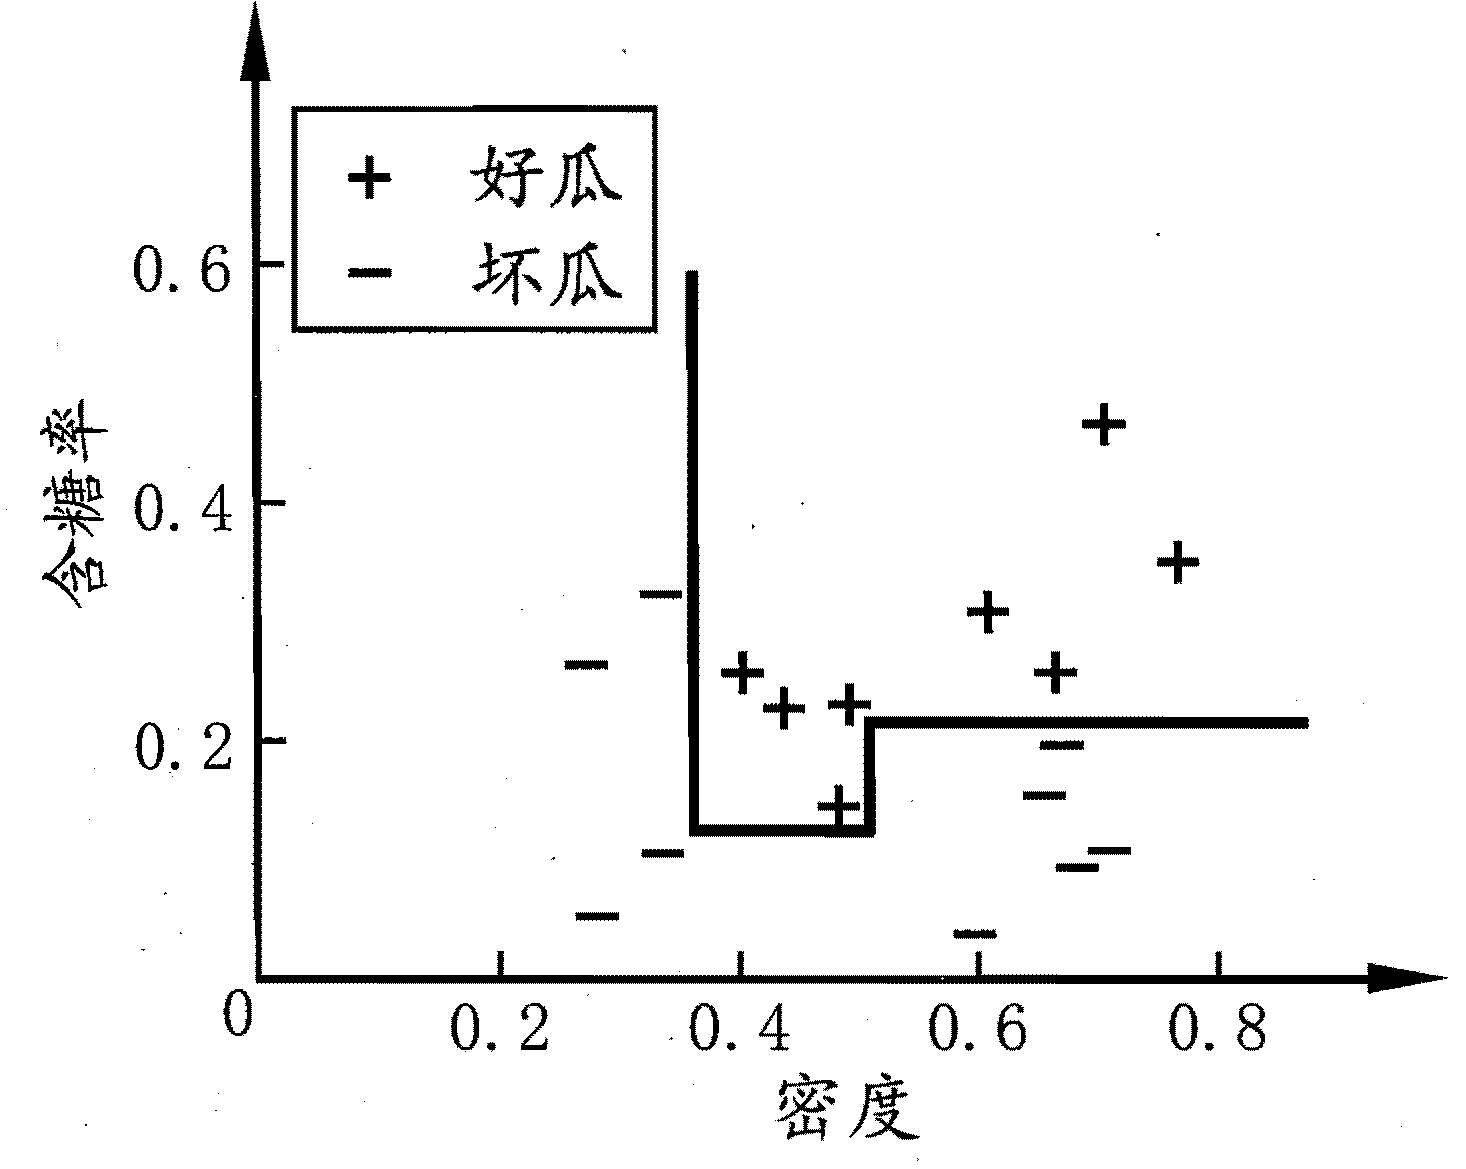
\includegraphics[scale=1,height=5.3cm]{../image/决策树对应的分类边界.png}
		\caption{决策树对应的分类边界}
	\end{figure}
	
	若能使用斜的划分边界,如图\ref{决策树复杂分类边界的分段近似}中红色线段所示,决策树模型将大为简化。“多变量决策树”就是能实现这样的“斜划分”甚至更复杂划分的决策树。
	
	在多分类决策树中,非叶结点不再是仅针对某个属性,而是对属性的线性组合进行测试;换言之,每个非叶结点是一个形如 $\sum\limits_{i=1}^d w_ia_i=t$的线性分类器,其中 $w_i$ 是属性 $a_i$ 的权重,$w_i$ 和 $t$ 可在该结点包含的样本集和属性集上学得。
	
	\begin{figure}[!htb]
		\centering
		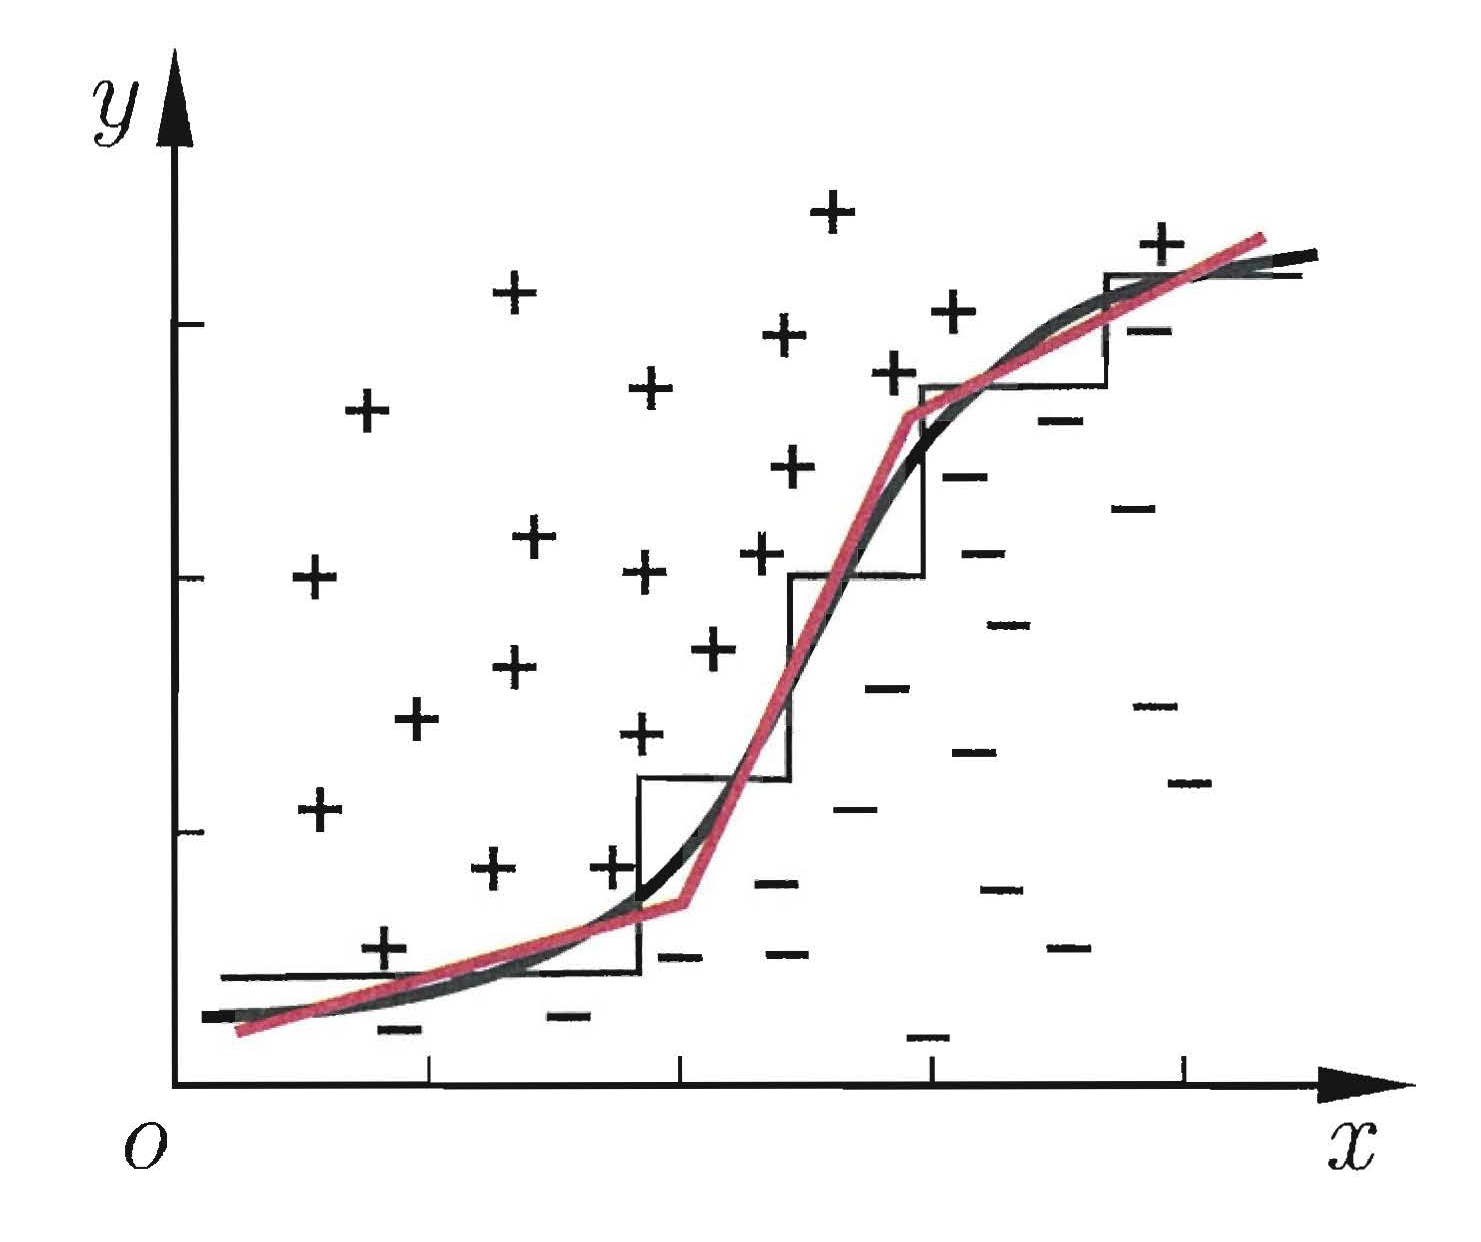
\includegraphics[scale=1,height=5.3cm]{../image/决策树复杂分类边界的分段近似.png}
		\caption{决策树复杂分类边界的分段近似}
		\label{决策树复杂分类边界的分段近似}
	\end{figure}

	总之,在多变量决策树的学习过程中,不是为每个非叶结点寻找一个最优划分属性,而是试图建立一个合适的线性分类器。在此次实验中,我使用对率回归构建多变量决策树。
	
	\subsection{算法设计思路}
	
	\subsubsection{数据结构设计}
	
	这里使用\href{https://networkx.org}{NetworkX}创建树结构。
	
	NetworkX可赋予结点和边任意属性,这里为边和结点赋予属性label。如图\ref{数据结构设计},树的非叶结点的label标记选择划分的属性,叶结点label标记类别,边的label标记属性值。
	
	\begin{figure}[!htb]
		\centering
		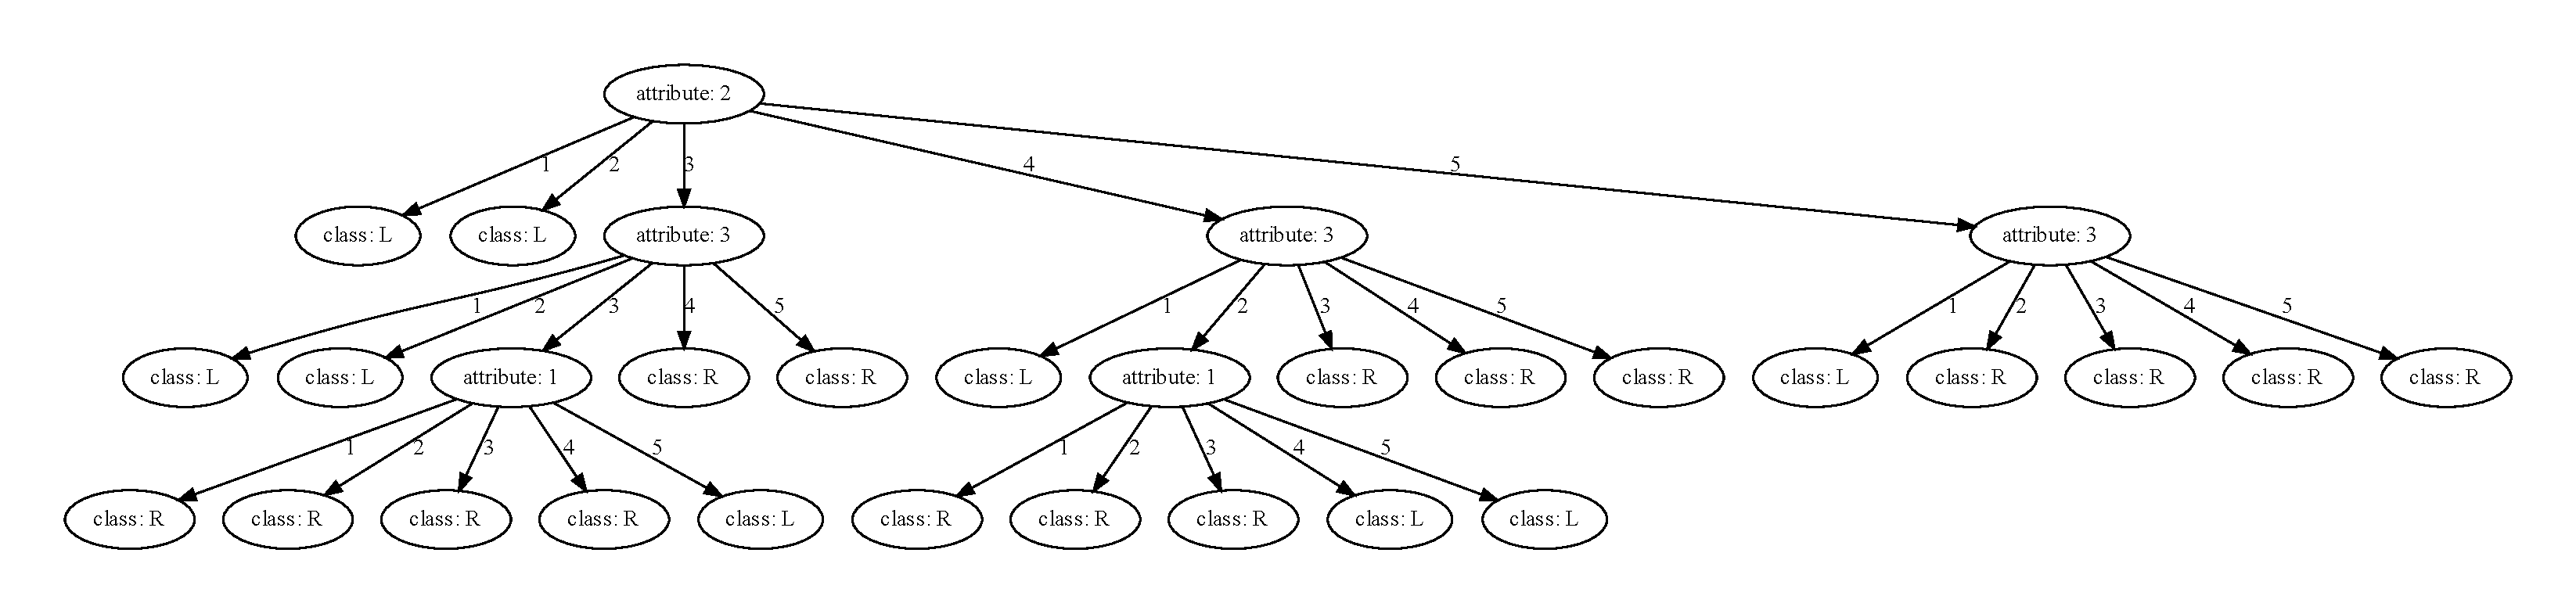
\includegraphics[scale=1,width=\textwidth]{../image/post_pruning-Gain-balance-scale.gv.pdf}
		\caption{数据结构设计}
		\label{数据结构设计}
	\end{figure}

	\subsubsection{建树过程}
	
	基于算法\ref{决策树学习基本算法},我们可以将其加以改造为算法\ref{决策树学习DFS},实现建树过程。递归的建树过程是DFS,我们可将其再改造为如算法\ref{决策树学习BFS}的BFS过程。
	
	\begin{algorithm}[!htb]
		\caption{决策树学习DFS}  
		\label{决策树学习DFS}
		\begin{algorithmic}[1]
			\Require  
			训练集 $D=\{(\bm{x}_1,y_1),(\bm{x}_2,y_2),\cdots,(\bm{x}_m,y_m)\}$;属性集 $A=\{a_1,a_2,\cdots,a_d\}$;当前结点索引 $cur$。
			\Function{TreeGenerate}{$D$, $A$, $cur$}
				\If{$D$ 中样本全属于同一类别 $C$}
					\State 将 $cur$ 标记为 $C$ 类叶结点,其label为 $C$;
					\Return
				\EndIf
				\If{$A\neq\varnothing$ \textbf{OR} $D$ 中样本在 $A$ 上取值相同}
					\State 将cur标记为叶结点,其label标记为 $D$ 中样本最多的类;
					\Return
				\EndIf
				\State 从 $A$ 中选择最优划分属性 $a_\ast$;
				\State 将cur的label标记为 $a_\ast$;
				\For{$a_\ast$的每个值 $a_\ast^v$}
					\State 为 $cur$ 生成一个分支结点 $nxt$;令 $D_v$ 表示 $D$ 中在 $a_\ast$ 上取值为 $a_\ast^v$ 的样本子集;
					\If{$D_v$为空}
						\State 将 $nxt$ 标记为叶结点,其label为 $D_v$ 中样本最多的类;
						\State 建边 $(cur, nxt, \text{label}=a_\ast)$
						\Return
					\Else
						\State \Call{TreeGenerate}{$D_v$, $A\ \backslash\ \{a_\ast\}$, $nxt$}
						\State 建边 $(cur, nxt, \text{label}=a_\ast)$
					\EndIf
				\EndFor
			\EndFunction
		\end{algorithmic}  
	\end{algorithm}

	\begin{algorithm}[!htb]
		\caption{决策树学习BFS}  
		\label{决策树学习BFS}
		\begin{algorithmic}[1]
			\Require  
			训练集 $D_0=\{(\bm{x}_1,y_1),(\bm{x}_2,y_2),\cdots,(\bm{x}_m,y_m)\}$;初始属性集 $A_0=\{a_1,a_2,\cdots,a_d\}$。
			\Function{TreeGenerate}{$D_0$, $A_0$, $cur_0$}
				\State \textbf{define} 搜索队列 $Q$;
				\State 初始化决策树,加入唯一的结点,索引为1;
				\State \textbf{push} $(D_0,A_0,1)$ \textbf{to} $Q$
				\While{$Q$ 非空}
					\State $(D,A,cur)\gets$ \textbf{front of} $Q$;
					\State \textbf{pop} $Q$;
					\If{$D$ 中样本全属于同一类别 $C$}
						\State 将 $cur$ 标记为 $C$ 类叶结点,其label为 $C$;
						\textbf{continue}	
					\EndIf
					\If{$A\neq\varnothing$ \textbf{OR} $D$ 中样本在 $A$ 上取值相同}
						\State 将cur标记为叶结点,其label标记为 $D$ 中样本最多的类;
						\textbf{continue}
					\EndIf
					\State 从 $A$ 中选择最优划分属性 $a_\ast$;
					\State 将cur的label标记为 $a_\ast$;
					\For{$a_\ast$的每个值 $a_\ast^v$}
						\State 为 $cur$ 生成一个分支结点 $nxt$;令 $D_v$ 表示 $D$ 中在 $a_\ast$ 上取值为 $a_\ast^v$ 的样本子集;
						\If{$D_v$为空}
							\State 将 $nxt$ 标记为叶结点,其label为 $D_v$ 中样本最多的类;
							\State 建边 $(cur, nxt, \text{label}=a_\ast)$
							\textbf{continue}
						\Else
							\State 建边 $(cur, nxt, \text{label}=a_\ast)$
							\State \textbf{push} $(D_v,A\ \backslash\ \{a_\ast\}, nxt)$ \textbf{to} $Q$
						\EndIf
					\EndFor
				\EndWhile
			\EndFunction
		\end{algorithmic}  
	\end{algorithm}

	\subsubsection{多变量决策树}
	
	在本次实验中,结点上用对数几率回归作为线性分类器,对决策树结点上的样本进行二分类。如算法\ref{多变量决策树}所述,二分类后的样本会产生两个分支结点,若分支结点上的样本属于同一类别,或 $D$ 中样本不可进行二分类,则结束递归;否则继续扩展分支结点。
	
	\begin{algorithm}[!htb]
		\caption{多变量决策树}  
		\label{多变量决策树}
		\begin{algorithmic}[1]
			\Require  
			训练集 $D=\{(\bm{x}_1,y_1),(\bm{x}_2,y_2),\cdots,(\bm{x}_m,y_m)\}$;属性集 $A=\{a_1,a_2,\cdots,a_d\}$;当前结点索引 $cur$。
			\Function{TreeGenerate}{$D$, $A$, $cur$}
				\If{$D$ 中样本全属于同一类别 $C$}
					\State 将 $cur$ 标记为 $C$ 类叶结点,其label为 $C$;
					\Return
				\EndIf
				\State 使用对率回归进行二分类,得到两个子集 $D_1$ 和 $D_2$
				\If{$D_1=\varnothing$ \textbf{OR} $D_2=\varnothing$}
					\State 将 $cur$ 标记为叶结点,其label标记为 $D$ 中样本最多的类;
					\Return
				\EndIf
				\State 生成结点 $nxt_1$ 表示子集 $D_1$
				\State 生成结点 $nxt_2$ 表示子集 $D_2$
				\State 建边 $(cur,nxt_1)$
				\State 建边 $(cur,nxt_2)$
				\State\Call{TreeGenerate}{$D_1$,$nxt_1$}
				\State\Call{TreeGenerate}{$D_2$,$nxt_2$}
			\EndFunction
		\end{algorithmic}  
	\end{algorithm}

	\subsubsection{预测方法}
	
	决策树学习完成后,可对样本进行预测。在预测样本真实类别时,从根结点出发,根据结点标记的划分属性,走对应划分属性值的边,到达子结点。
	
	\begin{figure}[!htb]
		\centering
		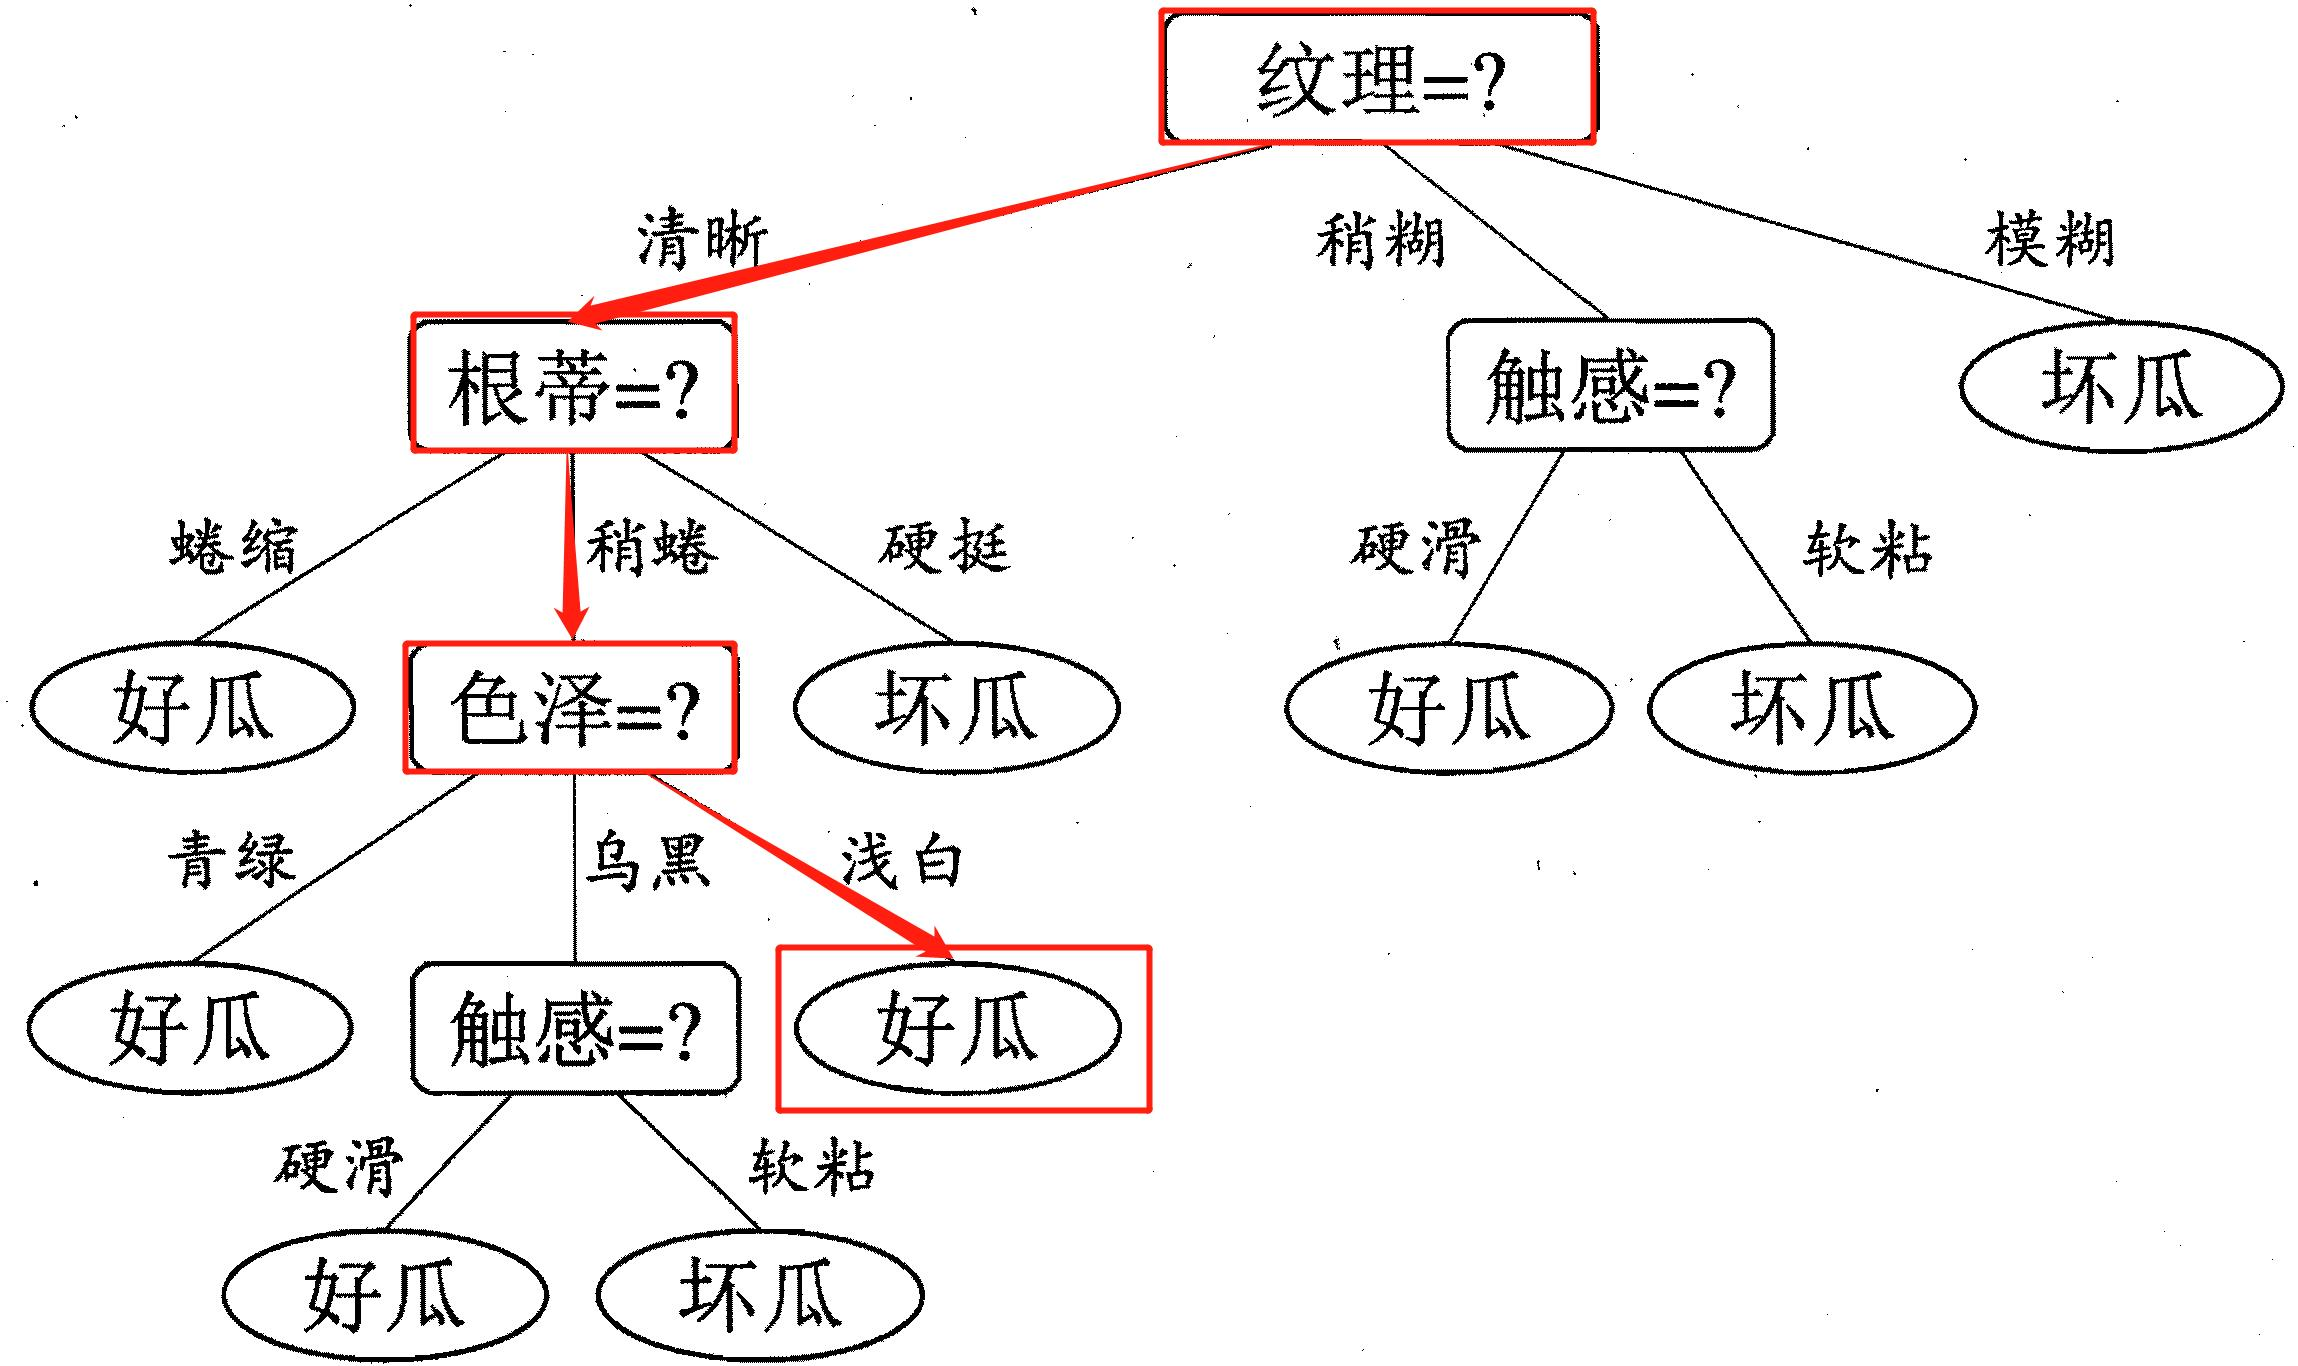
\includegraphics[scale=1,height=6cm]{../image/预测结果举例.jpg}
		\caption{样本预测举例}
		\label{样本预测举例}
	\end{figure}

	以图\ref{样本预测举例}为例,一个西瓜的纹理清晰、根蒂稍蜷、色泽浅白,它的预测结果是好瓜。其决策路径在图\ref{样本预测举例}中用红色标出。
	
	\subsubsection{预剪枝}
	
	先剪枝在建树过程中进行,使用BFS方式构建较为方便。在算法\ref{决策树学习BFS}生成分支结点前,需要暂时生成两棵树 $T_s$ 和 $T_d$,其中 $T_s$ 为以标记当前结点 $cur$ 为叶结点的树,$T_d$ 为生成 $cur$ 分支结点的树。使用测试集对两棵决策树进行性能评估,若 $T_d$ 的正确率更高,则生成分支结点继续搜索,否则在当前结点停止扩展。 
	
	\subsubsection{后剪枝}
	
	后剪枝在建树过后进行,自底向上标记深度最大的非叶结点为出现个数最多的类,并删除其叶结点。
	
	为了做到自底向上删除结点,我们需要在建树后对其再进行一次DFS,得到每个结点的深度,定义结点 $i$ 的深度为 $d_i$,根结点的深度为1,则
	
	\begin{equation}
		d_{\text{son}_i}=d_i+1
	\end{equation}

	得到深度数组后,将结点按照深度降序排列,依次队深度最大的非叶结点剪枝即可;整个后剪枝过程会依次删除深度最大的结点,但不影响其它结点的深度,因此深度数组无需在对一个结点进行一次剪枝后重新求。若对一个深度较大的结点进行剪枝后,能增大测试集的正确率,则对此结点剪枝。
	
	\subsection{核心代码详解}
	
	\subsubsection{函数简介}
	
	\begin{table}[!htb]
		\centering
		\begin{tabular}{|l|l|}
			\hline
			函数名&功能\\
			\hline
			split\_data\_and\_target(D)&将样本集D分割为属性集X和真实标记y\\
			\hline
			Ent(D)&计算D的信息熵\\
			\hline
			get\_Dv(D, a, v)&获得样本D中属性a取值为v的子集\\
			\hline
			Gain(D, a, class\_dicts)&计算信息增益\\
			\hline
			Gini(D)&计算基尼值\\
			\hline
			Gini\_index(D, a, class\_dicts)&计算基尼系数\\
			\hline
			count\_value\_num(X, v)&矩阵X中包含行向量v的个数\\
			\hline
			get\_greatest\_split\_attribute(D, A, solver='Gini\_index')&选择最优划分属性\\
			\hline
		\end{tabular}
	\end{table}
	
	\subsubsection{数据读取}
	
	在此次实验中,我使用了\href{https://archive.ics.uci.edu/ml/datasets/Lymphography}{Lymphography}、\href{https://archive.ics.uci.edu/ml/datasets/balance+scale}{
		Balance Scale}、\href{https://archive.ics.uci.edu/ml/datasets/Tic-Tac-Toe+Endgame}{
		Tic-Tac-Toe}、\href{https://archive.ics.uci.edu/ml/datasets/Ionosphere}{
		Ionosphere}四个UCI数据集,根据不同数据集的格式,我专门定义了读取数据的程序DataLoader。
	
	DataLoader读取不同的数据集,并将数据集转换为统一的格式提供给数据集使用者。DataLoader提供的数据集用NumPy的ndarray存储,每一行代表一个样本,最后一列为样本的真实值;DataLoader还提供一个字典class\_dicts,字典的key为属性、value为属性可取的值。
	
	\lstinputlisting[style=Python]{../code/core/数据读取.txt}
	
	\subsubsection{决策树学习}
	
	依据算法\ref{决策树学习DFS},未剪枝决策树学习的过程如下。代码中,叶结点的标记用“class: ”开头,表示类别;非叶结点的标记用“attribute: ”开头,表示划分属性;边上标记属性值。
	\lstinputlisting[style=Python]{../code/core/决策树学习.txt}
	
	\subsubsection{多变量决策树}
	
	依据算法\ref{多变量决策树},基于对率回归的多变量决策树学习过程如下。代码中,直接将样本集合拆分为参数矩阵 $X$ 和真实标记向量 $y$ 传入。叶结点的标记用“class: ”开头,表示类别;非叶结点的标记用于表示对率回归分类器的参数值 $\bm{w}$ 和 $b$;基于对率回归的“二分类”特性,每个非叶结点产生两个分支,分别为 $\bm{w}^\mathrm{T}\bm{x}+b>0$ 和 $\bm{w}^\mathrm{T}\bm{x}+b\leqslant0$。
	
	\lstinputlisting[style=Python]{../code/core/多变量决策树.txt}
	
	\subsubsection{预剪枝}
	
	预剪枝在建树过程中进行,这里使用BFS实现。在算法\ref{决策树学习BFS}的基础上,建树过程增加了准确性的判断,仅当继续产生分支结点得到的决策树准确率更高,才继续搜索过程。
	\lstinputlisting[style=Python]{../code/core/预剪枝.txt}
	
	\subsubsection{后剪枝}
	
	后剪枝在建树过后进行。首先需要调用get\_depth函数获得每个结点的深度,然后从深度大的非叶结点开始,依次对非叶结点进行剪枝。
	
	\lstinputlisting[style=Python]{../code/core/后剪枝.txt}
	
	\subsection{实验结果分析}
	
	使用\href{https://archive.ics.uci.edu/ml/datasets/Lymphography}{Lymphography}、\href{https://archive.ics.uci.edu/ml/datasets/balance+scale}{
		Balance Scale}、\href{https://archive.ics.uci.edu/ml/datasets/Tic-Tac-Toe+Endgame}{
		Tic-Tac-Toe}三个UCI数据集对ID3算法和CART算法进行测试。
	
	针对每个数据集训练一棵决策树,取数据集的80\%作为训练集,其余作为测试集,测试集的准确率如表\ref{ID3结果}和表\ref{CART结果}。可以发现,只有Tic-Tac-Toe数据集,预剪枝后的准确率较未剪枝的决策树低,其余的剪枝操作都能使得预测结果提高。对比图\ref{Tic-Tac-Toe数据集预剪枝ID3决策树}和图\ref{Tic-Tac-Toe数据集后剪枝ID3决策树}可看出,Tic-Tac-Toe数据集的后剪枝决策树相比预剪枝决策树保留了更多的分支。可初步得出结论:后剪枝决策树的欠拟合风险小,泛化性能优于预剪枝决策树。由于后剪枝过程是在完成决策树之后进行的,并且要自底向上地对树中的所有非叶结点进行逐一考查,因此其训练时间开销比未剪枝决策树和预剪枝决策树都大得多。
	
	\begin{table}[!htb]
		\begin{minipage}[b]{.46\textwidth}
			\centering
			\begin{tabular}{l|l|l|l}
				\hline
				& 未剪枝   & 预剪枝   & 后剪枝   \\
				\hline
				Lymphography        & 0.667 & 0.767 & 0.767 \\
				\hline
				Balance Scale       & 0.664 & 0.704 & 0.704 \\
				\hline
				Tic-Tac-Toe & 0.875 & 0.703 & 0.943 \\   
				\hline
			\end{tabular}
			\caption{ID3结果}
			\label{ID3结果}
		\end{minipage}
		\hfill
		\begin{minipage}[b]{.46\textwidth}
			\centering
			\begin{tabular}{l|l|l|l}
				\hline
				& 未剪枝   & 预剪枝   & 后剪枝   \\
				\hline
				Lymphography &0.633 &0.767 &0.767 \\
				\hline
				Balance Scale & 0.664&0.704 & 0.704 \\
				\hline
				Tic-Tac-Toe &0.875&0.703 & 0.943\\   
				\hline
			\end{tabular}
			\caption{CART结果}
			\label{CART结果}
		\end{minipage}
	\end{table}

	以Tic-Tac-Toe数据集为例,图\ref{Tic-Tac-Toe数据集未剪枝ID3决策树}为未剪枝决策树,图\ref{Tic-Tac-Toe数据集预剪枝ID3决策树}为预剪枝的决策树,图\ref{Tic-Tac-Toe数据集后剪枝ID3决策树}为后剪枝的决策树。可以发现,剪枝后的决策树不仅结点数和深度更小,能够提高样本的预测速度;基于表\ref{ID3结果}和\ref{CART结果},其准确率也会提高。
	
	\begin{figure}[!htb]
		\centering
		
\includegraphics[scale=1,width=\textwidth]{../image/normal-Gain-tic-tac-toe.gv.pdf}
		\caption{Tic-Tac-Toe数据集未剪枝ID3决策树}
		\label{Tic-Tac-Toe数据集未剪枝ID3决策树}
	\end{figure}

	\begin{figure}[!htb]
		\centering
		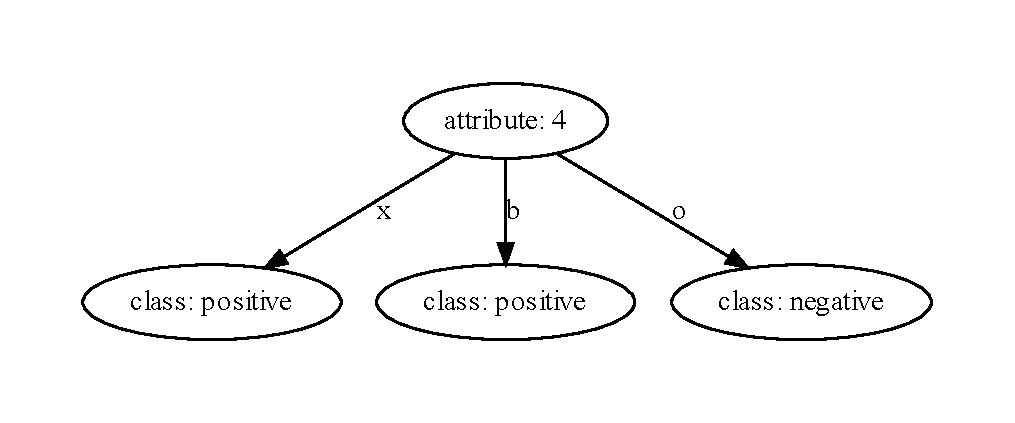
\includegraphics[scale=1,height=3.8cm]{../image/pre_pruning-Gain-tic-tac-toe.gv.pdf}
		\caption{Tic-Tac-Toe数据集预剪枝ID3决策树}
		\label{Tic-Tac-Toe数据集预剪枝ID3决策树}
	\end{figure}
	
	\begin{figure}[!htb]
		\centering
		
\includegraphics[scale=1,width=\textwidth]{../image/post_pruning-Gain-tic-tac-toe.gv.pdf}
		\caption{Tic-Tac-Toe数据集后剪枝ID3决策树}
		\label{Tic-Tac-Toe数据集后剪枝ID3决策树}
	\end{figure}

	使用\href{https://archive.ics.uci.edu/ml/datasets/Ionosphere}{
		Ionosphere}数据集对基于对率回归的多变量决策树进行测试,其准确率为0.944。未剪枝多变量决策树准确率就已经足够高,且决策树的结点数和深度也不大。多变量决策树的优点在于,其斜向的分类边界能够加快分类速度,提高分类准确率。
	
	\begin{figure}[!htb]
		\centering
		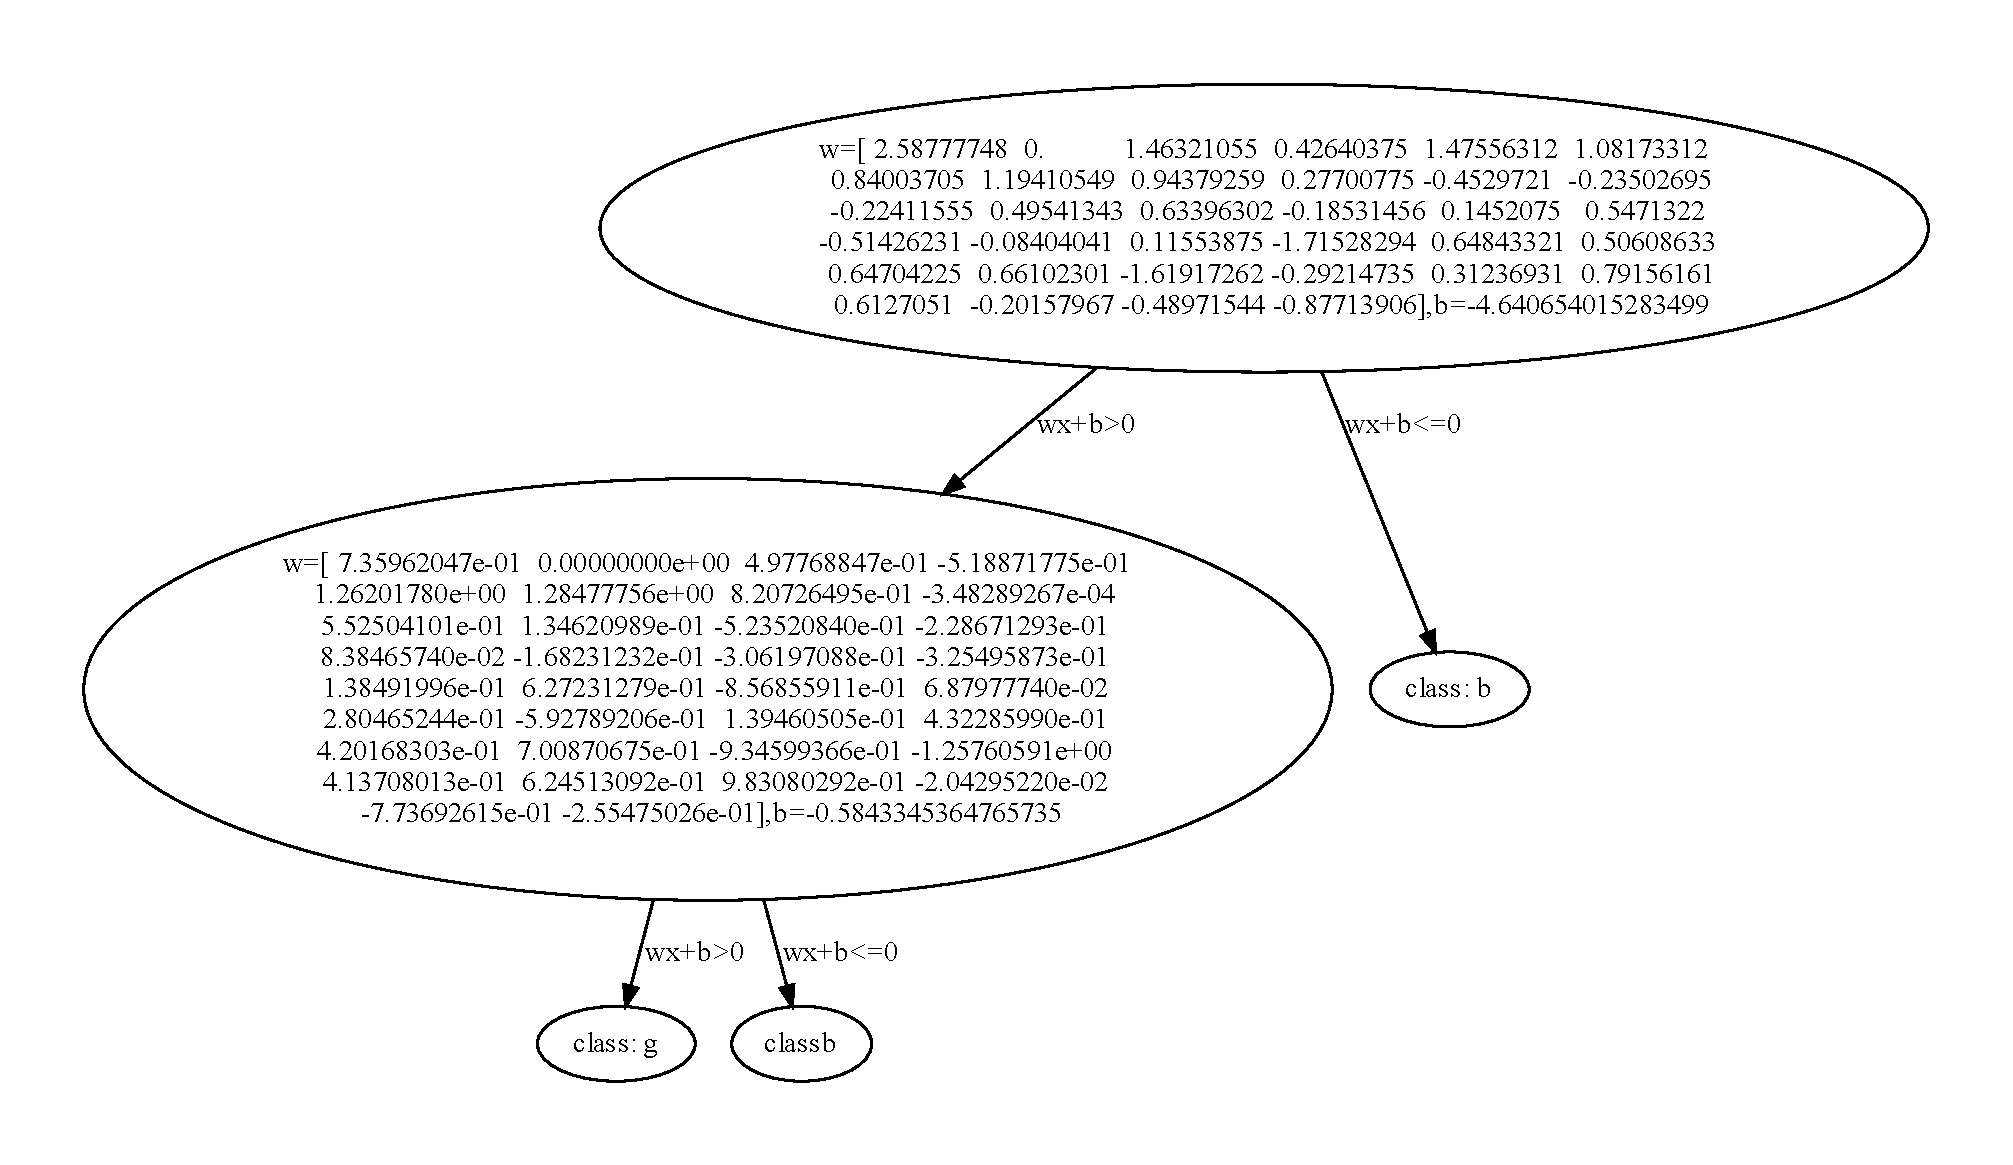
\includegraphics[scale=1,width=\textwidth]{../image/multivariate-normal-ionosphere.gv.pdf}
		\caption{Ionosphere数据集基于对率回归的决策树}
		\label{Ionosphere数据集基于对率回归的决策树}
	\end{figure}
	
	\subsection{学习收获}
	
	在此次实验中,我尝试实现了多个决策树学习算法,包括ID3、CART、多变量决策树等,并对决策树进行了剪枝操作,得出了“后剪枝较预剪枝”更优的结论。此次实验只利用决策树完成了分类任务,还可以进一步使用决策树完成回归任务。个人认为,决策树逻辑简单、易实现、没有很强的数学性,但是所占的空间复杂度有一些大。
	
	相比自己实现的决策树学习算法,sklearn提供的决策树学习算法处理了连续值和离散值,可控制决策树生长时的各类阈值,同时能借助graphviz画出决策树。如图\ref{iris数据集决策树},是利用sklearn生成的iris数据集决策树。
	
	\begin{figure}[!htb]
		\centering
		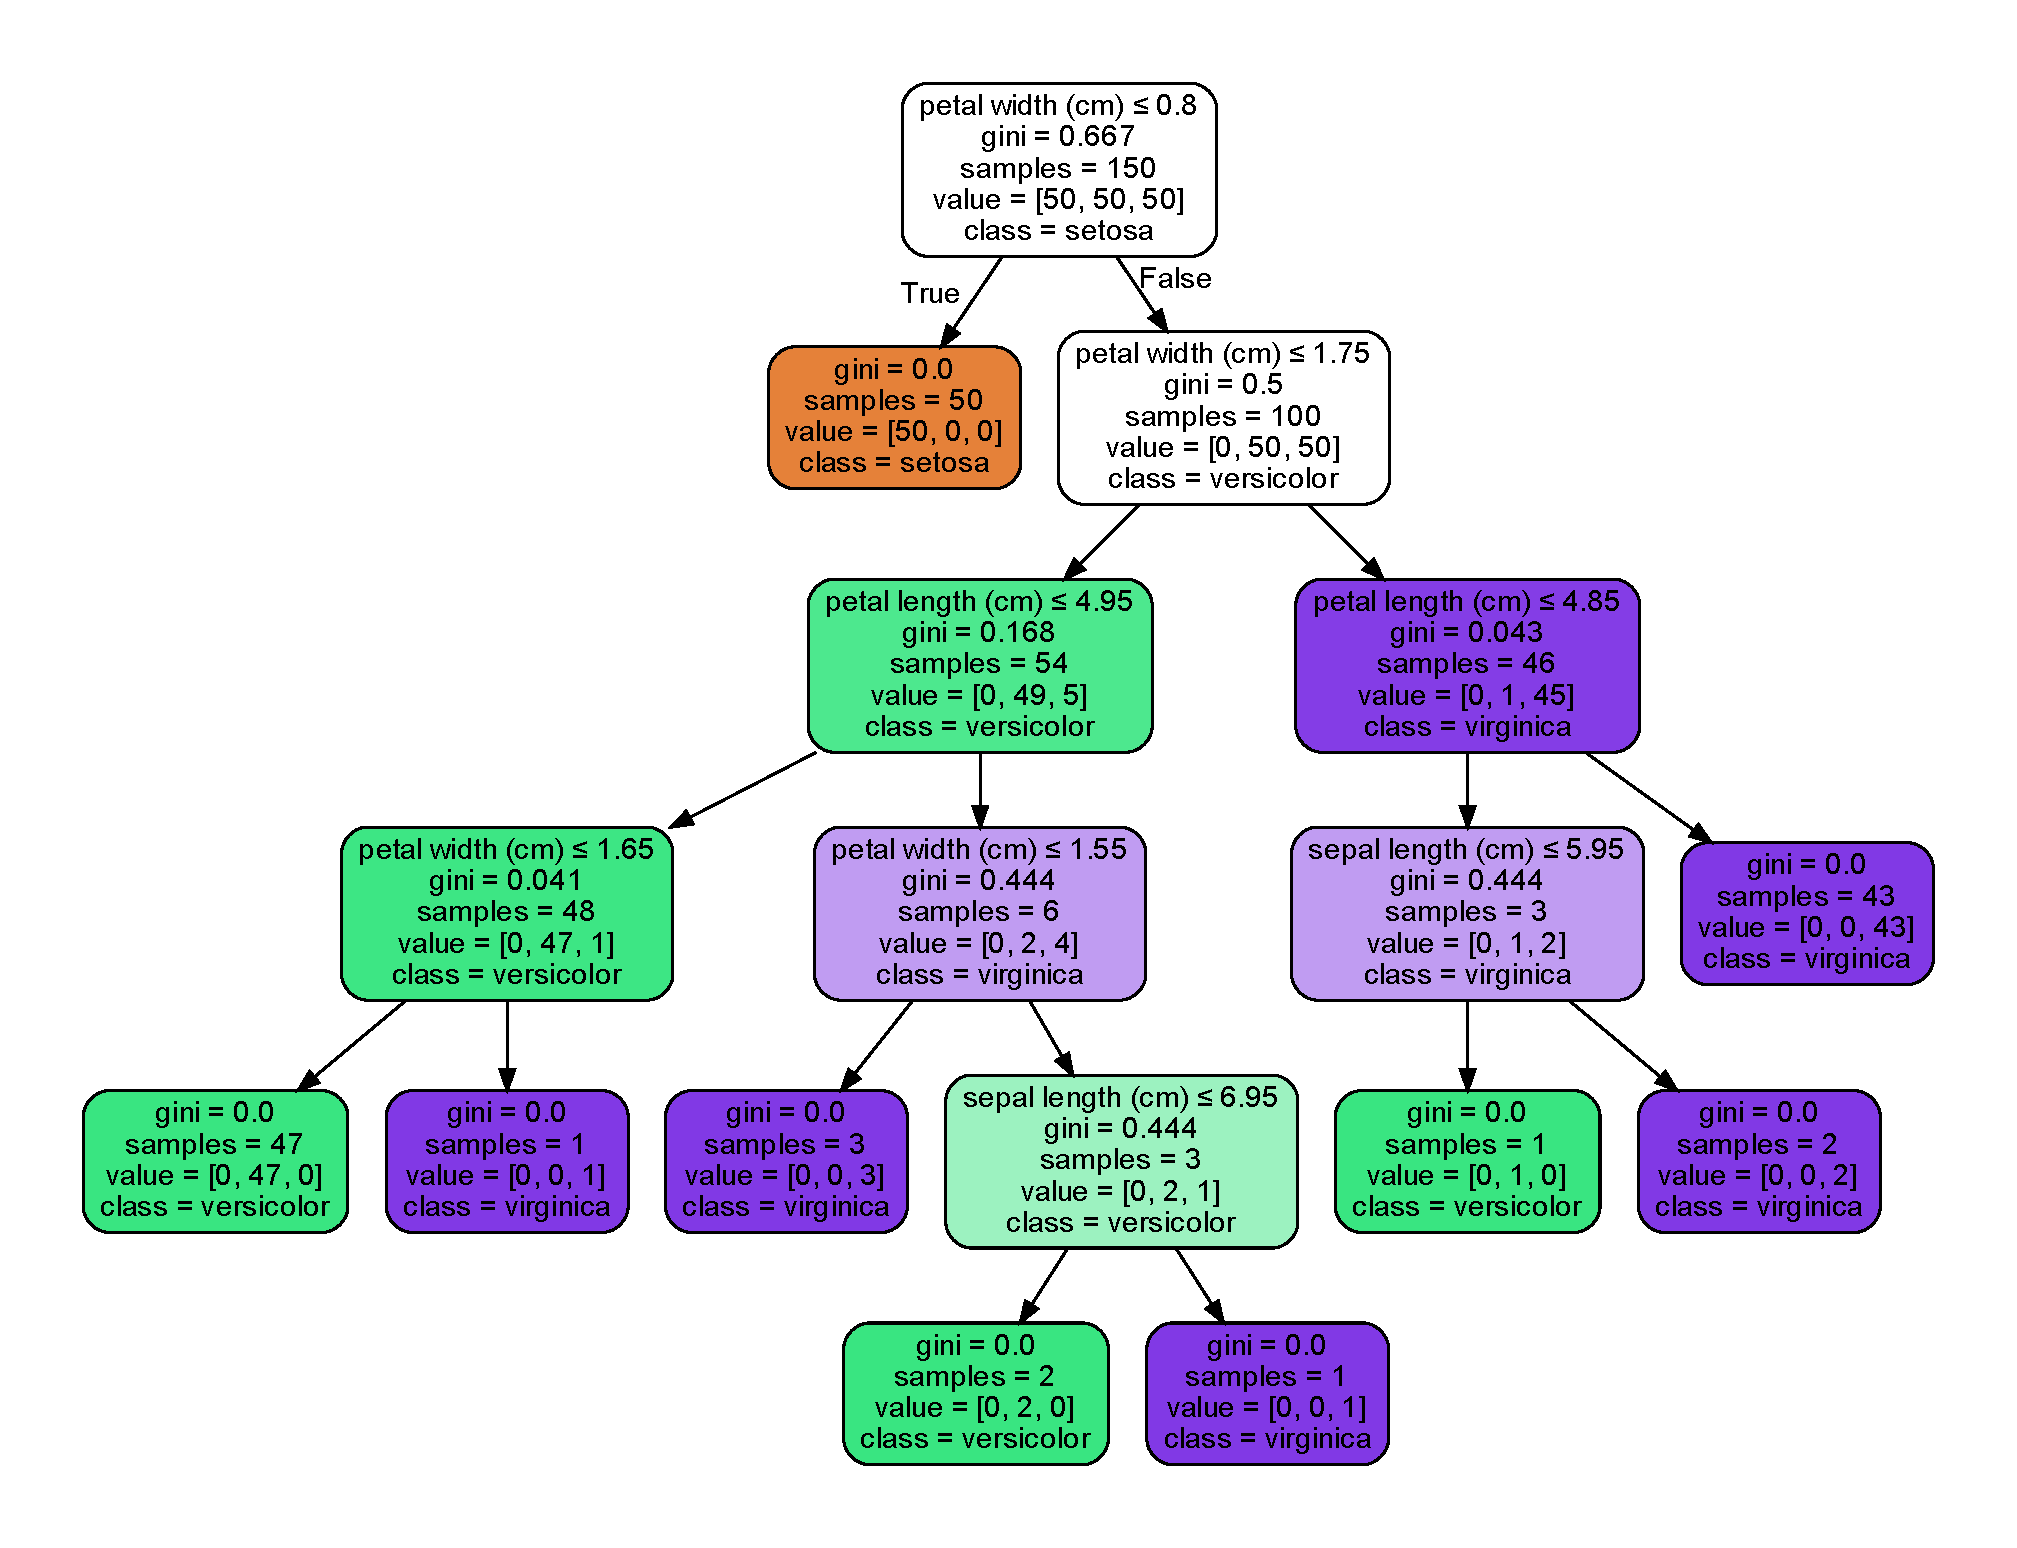
\includegraphics[scale=1,width=\textwidth]{../image/iris.gv.pdf}
		\caption{iris数据集决策树}
		\label{iris数据集决策树}
	\end{figure}
	
	\subsection{参考资料}   
	\begin{itemize}
		\item \href{https://scikit-learn.org.cn/view/89.html#1.10.1%20%E5%88%86%E7%B1%BB}{决策树分类(scikit-learn中文社区)}
		\item \href{https://scikit-learn.org.cn/view/784.html}{sklearn.tree.DecisionTreeClassifier(sckikit-learn中文社区)}
		\item 《机器学习》4.决策树;清华大学出版社;周志华
	\end{itemize}
	\section{习题2}
	
	\subsection{编程题目理解}
	题目要求:使用"队列"数据结构,以参数MaxDepth控制树的最大深度,写出使用非递归的决策树生成算法。
	算法\ref{决策树学习BFS}已经给出了非递归的,即广度优先的建树算法,对此加以改造即可。
	\subsection{算法设计思路}
	定义状态 $(cur,D,A,depth)$,分别表示当前结点编号、样本集合、属性集合、结点深度。相比算法\ref{决策树学习BFS},这里向BFS记录的状态中添加了“深度”这一状态。每次生成分支节点,都将新结点的深度在当前结点的基础上增加1,将新的结点加入队列。当结点的深度达到MaxDepth时,则停止搜索。
	\subsection{核心代码分析}
	在建树过程中,记录结点的深度,当深度达到MaxDepth则停止搜索。
	\lstinputlisting[style=Python]{../code/core/限制深度BFS.txt}
	\subsection{实验结果}
	使用西瓜数据集2.0学习得到的决策树如图\ref{MaxDepth决策树},其准确率为0.4286。
	\begin{figure}[!htb]
		\centering
		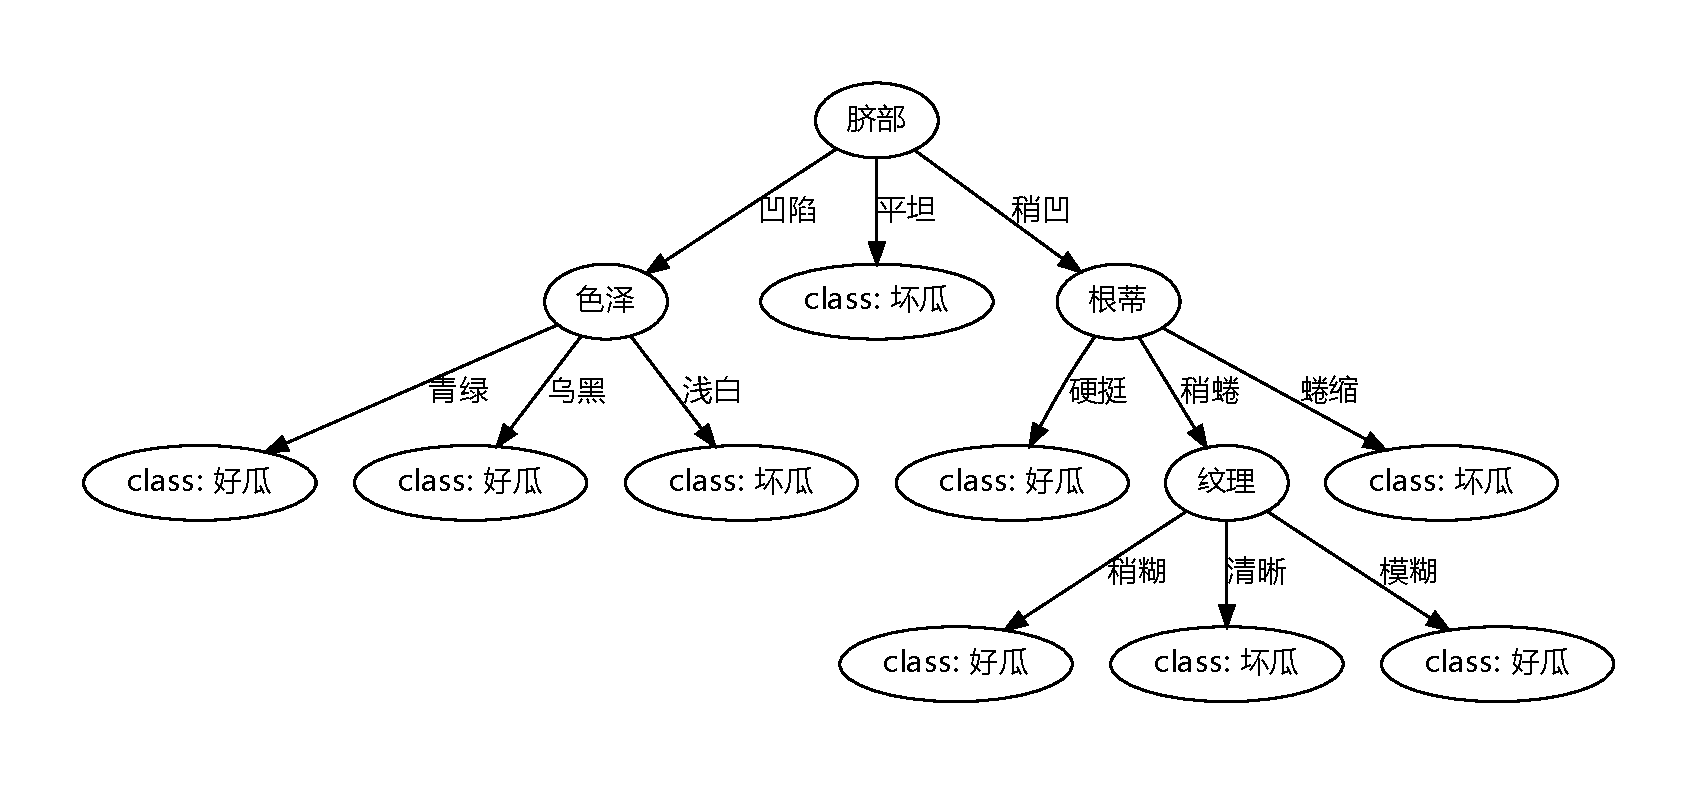
\includegraphics[scale=1,height=7cm]{../image/limit_MaxDepth-Gain-watermelon2.0.gv.pdf}
		\caption{限制结点深度得到的决策树}
		\label{MaxDepth决策树}
	\end{figure}
	\subsection{学习收获}
	构建决策树时限制结点的最大深度,能够有效减少递归的层数、加快决策树的学习速度,也避免了一些过拟合的风险;但是这本质上还是一种类似预剪枝的策略,且没有剪枝时的准确率检验。
	
	\section{习题3}
	\subsection{编程题目理解}
	题目要求:以参数MaxNode控制树的最大结点数,写出使用非递归的决策树生成算法。
	算法\ref{决策树学习BFS}已经给出了非递归的,即广度优先的建树算法,对此加以改造即可。
	\subsection{算法设计思路}
	定义状态 $(cur,D,A)$,分别表示当前结点编号、样本集合、属性集合,限制条件“结点数”由NetworkX维护。每次生成分支节点,都考虑生成分支结点后决策树结点是否会超过MaxNode;若不超过,则生成分支结点;否则,标记当前结点为样本中出现最多的种类,并停止搜索。
	\subsection{核心代码}
	在建树过程中,维护决策树的结点数,当扩展结点后结点数超过MaxNode则停止搜索。
	\lstinputlisting[style=Python]{../code/core/限制结点数BFS.txt}
	\subsection{实验结果分析}
	使用西瓜数据集2.0学习得到的决策树如图\ref{MaxNode决策树},其准确率为0.5714。
	\begin{figure}[!htb]
		\centering
		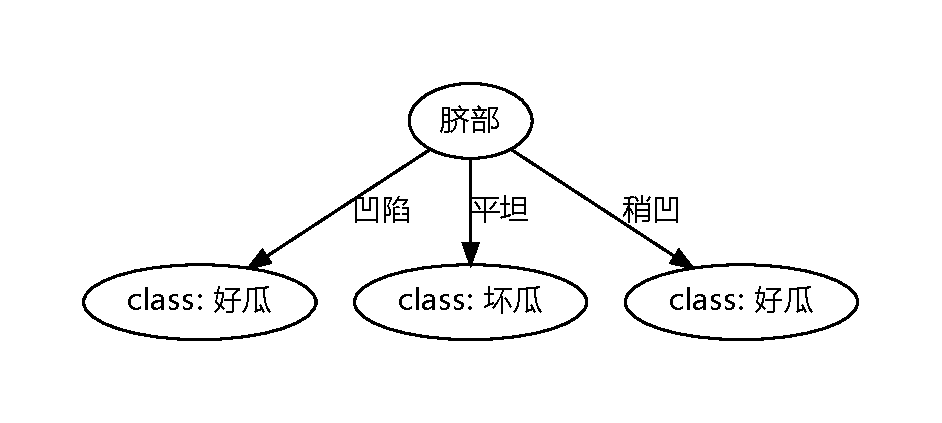
\includegraphics[scale=1,height=5cm]{../image/limit_MaxNode-Gain-watermelon2.0.gv.pdf}
		\caption{限制结点数得到的决策树}
		\label{MaxNode决策树}
	\end{figure}
	\subsection{学习收获}
	限制MaxDepth能有效减小树的深度,在预测样本值时能更快到达叶结点。限制MaxNode能有效减少决策树的空间复杂度。
	
	由于生成分支结点时,需要将一个属性的所有分支结点一次性生成,否则在预测样本时缺失属性值而导致无法到达叶结点;因此MaxNode取值不当时,可能出现生成分支结点后决策树结点数仅仅只超出MaxNode一些,使得当前结点无法继续搜索的情况。针对这种情况,不妨对MaxNode设置一个容错空间 $\epsilon$,即决策树可超出限制 $\epsilon$ 个结点。
\end{document}